\documentclass{article}
\usepackage[utf8]{inputenc}

\title{Image Preprocessing}
\author{Mihir Patel}
\date{January 2018}

\usepackage[letterpaper, margin=1in]{geometry}
\usepackage{natbib}
\usepackage{graphicx}
\usepackage{amsmath}
\usepackage{movie15}
\usepackage{hyperref}

\begin{document}

\maketitle

\section{Introduction}

So far we have talked about how machine learning and deep learning architectures can be applied to image related problems. We now will address certain preprocessing and data science techniques we can use to improve performance.

\section{Image Rescaling}
We aim to better normalize pixel values before feeding them into neural networks. If we feed in the raw values, they tend to be very high and varying (in most cases 0 to 255), which increases instability and forces the network to learn these artificial bounds in the first layer's weights. This is particularly difficult given the distance of this layer from the output so we instead rectify this with preprocessing.

\begin{enumerate}
  \item \textbf{Mean Subtraction:} Subtract the mean from each pixel value. This helps split the values evenly across zero, which is how networks typically transfer information.
  \item \textbf{Normalization/Whitening:} Subtract the mean and and divide by the standard deviation. This splits the values across zero and compresses the values to approximately -3 to 3, giving a better range of values.
\end{enumerate}

Sometimes, these two techniques are applied for each individual color channel instead of across the image if there is sizable variation within color channels.

\section{Image Generator}
When feeding in images to networks, we want to make the information learned as generalizable as possible. For example, if we see a cat upside down, the network should still recognize that a cat is there. To do this we use the Keras ImageDataGenerator. The data generator takes in all of the images and certain hyperparameters are set. It then produces batches of data to be fed into the network which are a blend of original images and modified images. The hyperparameters/modifications made by the generator are:

\begin{enumerate}
  \item \textbf{Shift:} Randomly shift image in x or y directions and fill empty space based on hyperparameter
  \item \textbf{Zoom:} Randomly zoom in or out on image and fill empty space based on hyperparameter
  \item \textbf{Rotation:} Randomly rotate image up to k degrees
  \item \textbf{Flip:} Flip image over x or y axis
\end{enumerate}

These all help the network better semantically learn the pattern in a more robust manner. However, as we shall later see with GANs, there are still many exploitable holes that remain even after these processing techniques.

\section{ImageNet}
By far the most popular and largest dataset for images is ImageNet. This competition has driven most advances in object classification, detection, and segmentation and boasts over 10,000,000 annotated data points. Most transfer learning is done off a model trained on ImageNet as it does general classification. The primary dataset in ImageNet consists of 100,000 various objects that are used for classification purposes.

\section{COCO: Common Object in Context}
COCO is another popular dataset that handles further analysis in images. As the figure below shows, COCO images contain pixel level segmentation so that advanced structures like Mask-RCNN and U-Nets can be trained. They also have 5 words associated with each image for image to text problems. There are approximately 200,000 annotated images.


\begin{center}
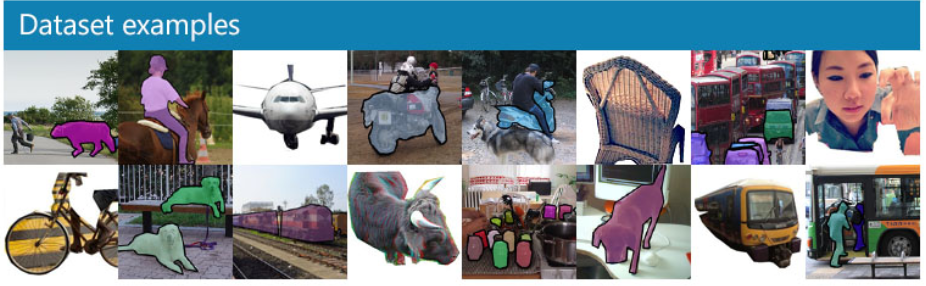
\includegraphics[scale=0.45]{coco.PNG}
\end{center}

\section{PASCAL VOC}
This is another dataset similar to COCO that has pixel level segmentation. It has about 30,000 images and is older (2012).

\section{mAP}
Something we haven't addressed is how we get error for image segmentation, namely for datasets like COCO and PASCAL. The specific metric used is mAP, or mean average precision. To calculate this, we first state that an object is successfully classified if the IoU (Intersection of Union), which is the overlap percentage of the proposed box and the correct box, is greater than .5. We then get AP, the average precision by:

$$ AP = \frac{True Positive}{True Positive + False Positive} $$

where true positive is a correctly classified object and a false positive is a proposed object that doesn't actually exist. The mAP is simply the mean of this statistic across all of the classes. A further extension of this is to get mAP[.5, .95], which means we first calculate mAP for each threshold between .5 to .95 at .05 increments (the thresold is used for IoU) and then average it. The higher thresholds are more rigorous for obvious reasons and have lower mAPs.

\end{document}
